\documentclass{beamer}
\usetheme{Copenhagen}
%\usetheme{Boadilla}
\usepackage{geometry}                % See geometry.pdf to learn the layout options. There are lots.
\usepackage{graphicx}
\usepackage{amssymb}
 \usepackage{feynmp}
 \usepackage{textpos}
 \usepackage{biblatex}
 \usepackage{bbold}
  \usepackage{ulem}
 \bibliography{foo}
  \DeclareGraphicsRule{*}{mps}{*}{} 
  % figures
  
 % \logo{
\includegraphics[height=1.2cm]{lhcblogo.jpg}\vspace{220pt}}
  
  
\usepackage{caption}
\usepackage{subfig}
\newcommand{\Lagr}{\mathcal{L}}
\setbeamertemplate{itemize item}{\scriptsize\raise1.25pt\hbox{\donotcoloroutermaths$\blacktriangleright$}}
\setbeamertemplate{itemize subitem}{\tiny\raise1.5pt\hbox{\donotcoloroutermaths$\square$}}
\setbeamertemplate{itemize subsubitem}{\tiny\raise1.5pt\hbox{\donotcoloroutermaths$\blacktriangleright$}}
\setbeamertemplate{enumerate item}{\insertenumlabel.}
\setbeamertemplate{enumerate subitem}{\insertenumlabel.\insertsubenumlabel}
\setbeamertemplate{enumerate subsubitem}{\insertenumlabel.\insertsubenumlabel.\insertsubsubenumlabel}
\setbeamertemplate{enumerate mini template}{\insertenumlabel}
\begin{document}

{


\title[Towards a Measurement of $V_{ub}$ with LHCb \hspace{2em}\insertframenumber/
\inserttotalframenumber]{Towards a Measurement of $V_{ub}$ with LHCb}
\author[William Sutcliffe]{
\includegraphics[height=1cm,width=1.5cm]{lhcblogo.jpg} \\ William Sutcliffe}

\date{\today}

 \frame{\titlepage

} 

\addtobeamertemplate{frametitle}{}{%
\begin{textblock*}{100mm}(.85\textwidth,-1cm)

\includegraphics[height=1cm,width=1.5cm]{lhcblogo.jpg}
\end{textblock*}}

 %%%%slide 1

 \frame{\frametitle{Outline} 
\begin{enumerate}
\setlength{\itemsep}{10pt}
\item Background and motivation.
\item Previous measurements.
\item $V_{ub}$ with LHCb
\item Initial generator level study
\end{enumerate}
}






 \frame{
 \frametitle{1 -  Current Status of $|V_{ub}|$}
 \begin{itemize}
  \item \normalsize{Semi-Leptonic B Decays:}
   \end{itemize}
   \hspace{1.cm} \footnotesize{Inclusive ($\bar{B} \rightarrow X_{u} l \bar{\nu}_{l}$)} \hspace{1cm}  \footnotesize{Exclusive ($\bar{B}_{0} \rightarrow \pi^{+} l \bar{\nu}_{l}$)}
    \begin{center} 
    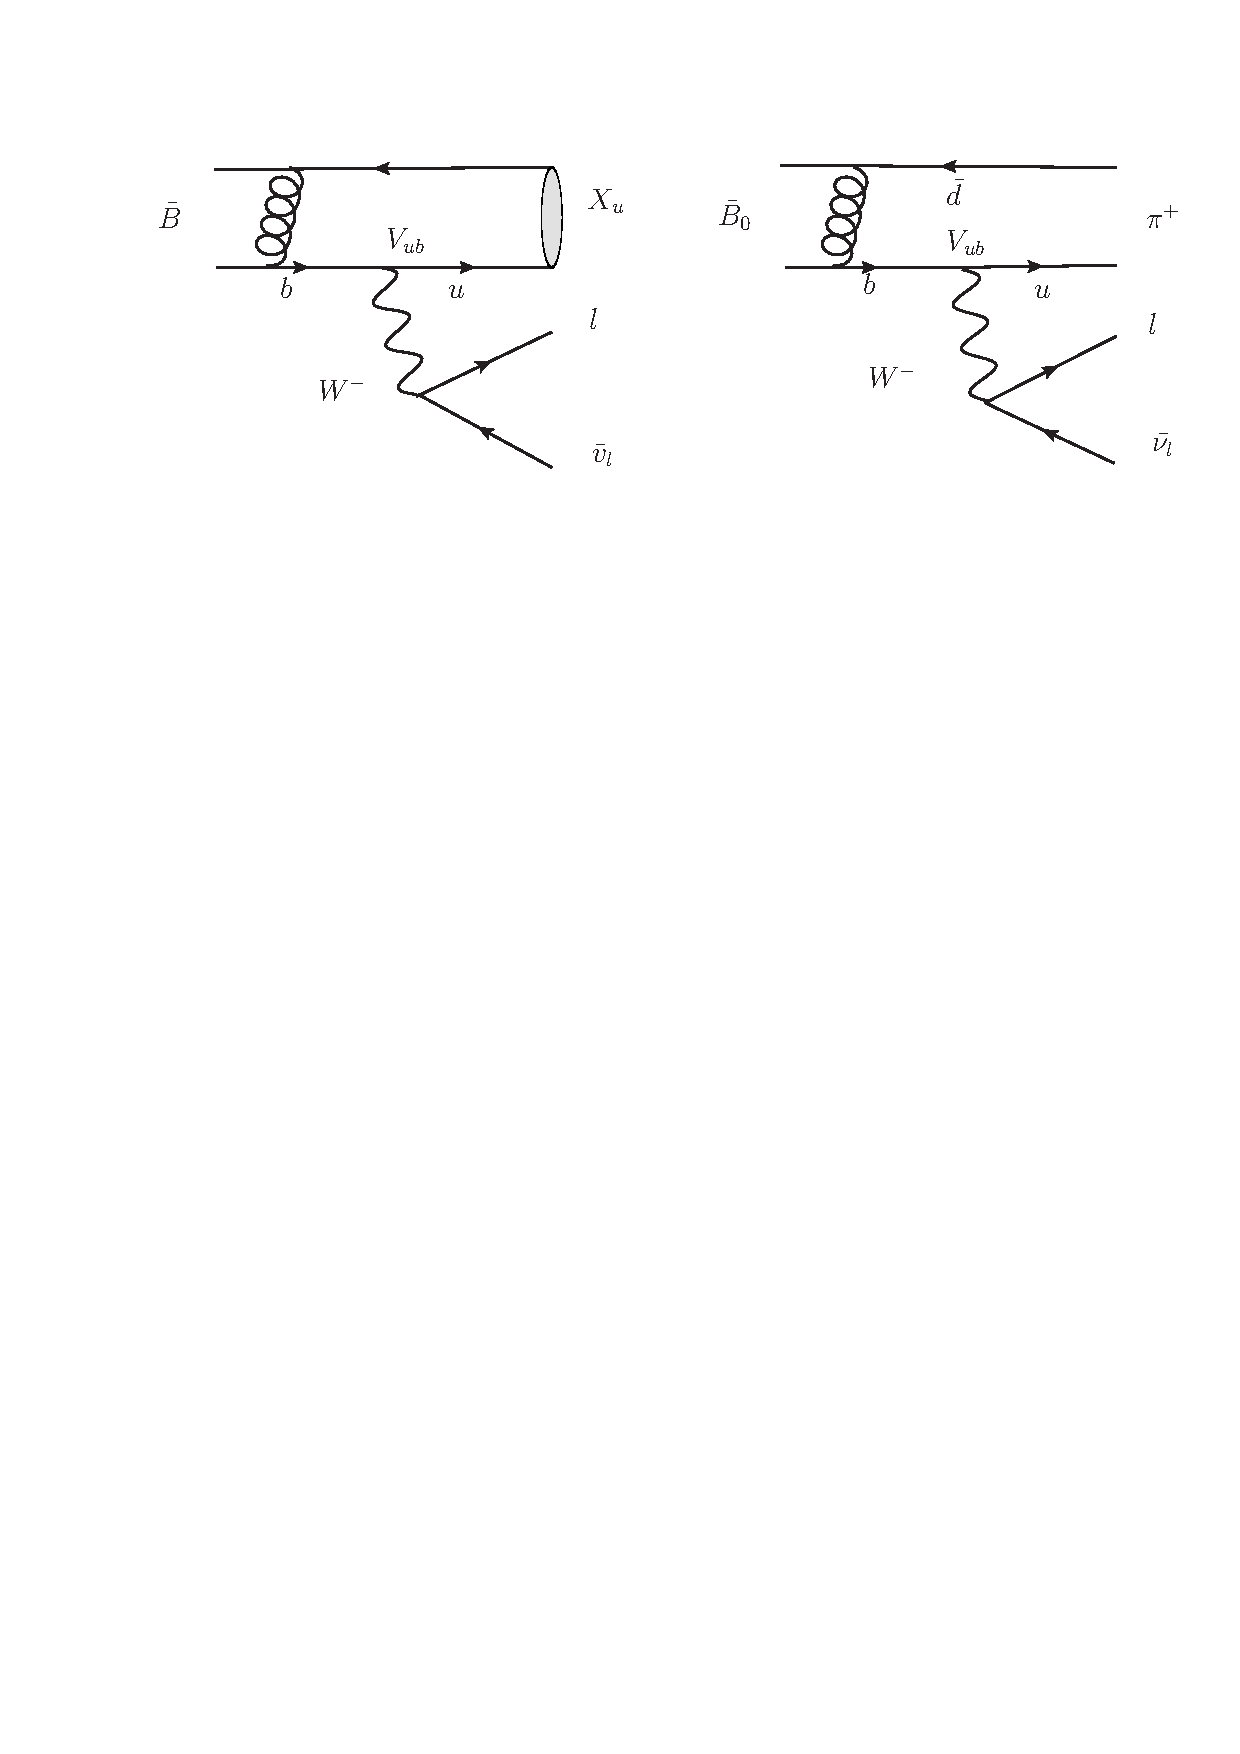
\includegraphics[trim = 15mm 215mm 0mm 25mm, clip, width=8cm]{incl_ex_feyn.pdf} 
        \end{center}
        \hspace{1.cm} \footnotesize{$|V_{ub}| = (4.41 \pm 0.15 ^{+ 0.15} _{-0.17}) \times 10^{-3}$} \hspace{0.3cm} \footnotesize{$|V_{ub}| = (3.23 \pm 0.31) \times 10^{-3}$}
  
  \vspace{0.1cm}
       \begin{itemize}
  \item \normalsize{Leptonic B decays ($B^{+} \rightarrow \tau^{+} \nu_{\tau}$):}
      \begin{center}
       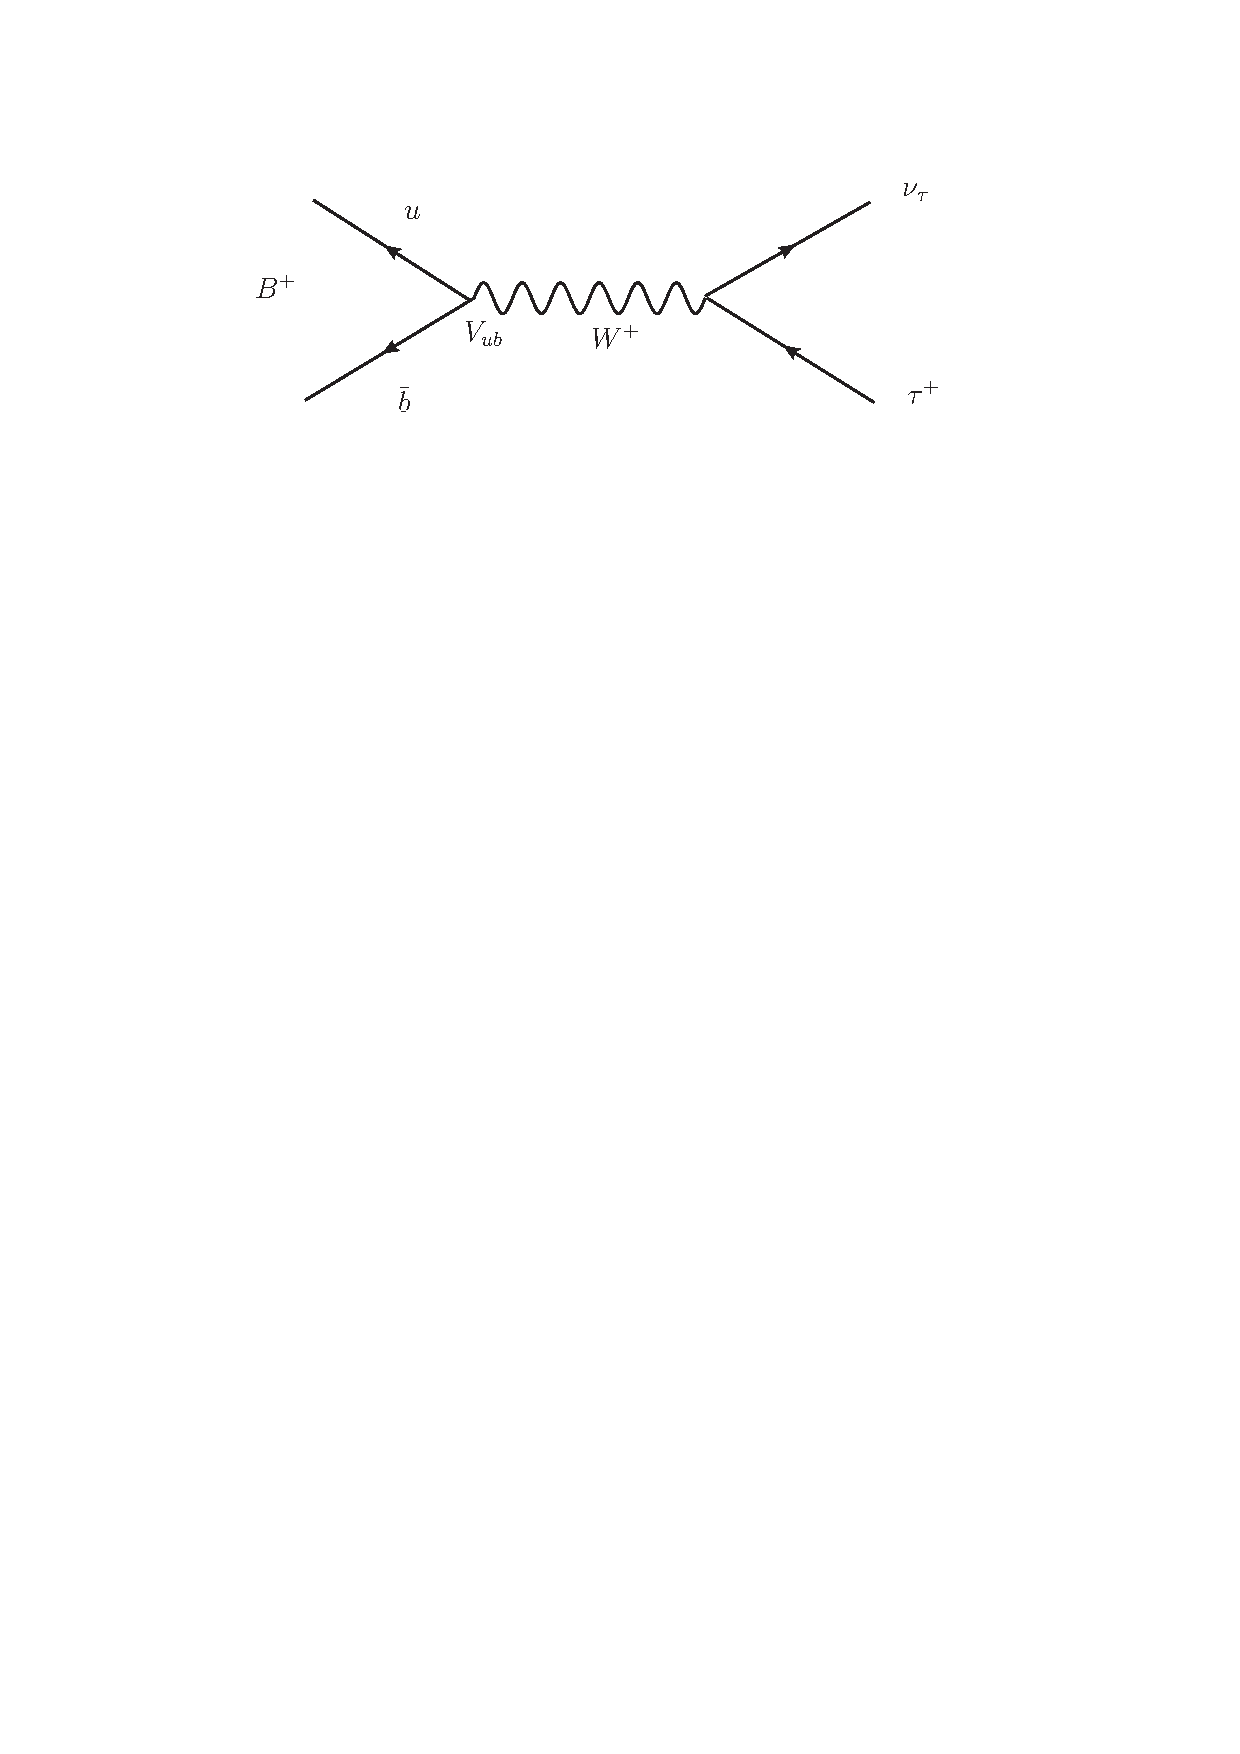
\includegraphics[trim = 15mm 215mm 0mm 30mm, clip, width=8cm]{lepfeyn.pdf} 
       \end{center}
   \end{itemize}
  

}




 \frame{
 \frametitle{1 - $|V_{ub}|$ Constraints on the Unitarity Triangle} 


            \begin{columns}[T]
   \begin{column}{.5\textwidth}
   \begin{itemize}

   \item \small{$V_{CKM} V_{CKM}^{\dagger} = \mathbb{1} $ $\implies$ \\ \vspace{0.2cm}
    $V_{ud} V^{*}_{ub} + V_{cd} V_{cb}^{*} + V_{td} V_{tb}^{*} = 0$ \\ \vspace{0.2cm} (+ 5 others)}
   \end{itemize}
   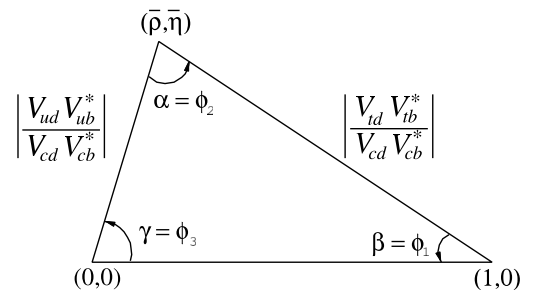
\includegraphics[width=1.0\textwidth]{UnitTri}
   
  \end{column}
      \begin{column}{.5\textwidth}
      % \footfullcite{gfgfg}
    
    \begin{center}
      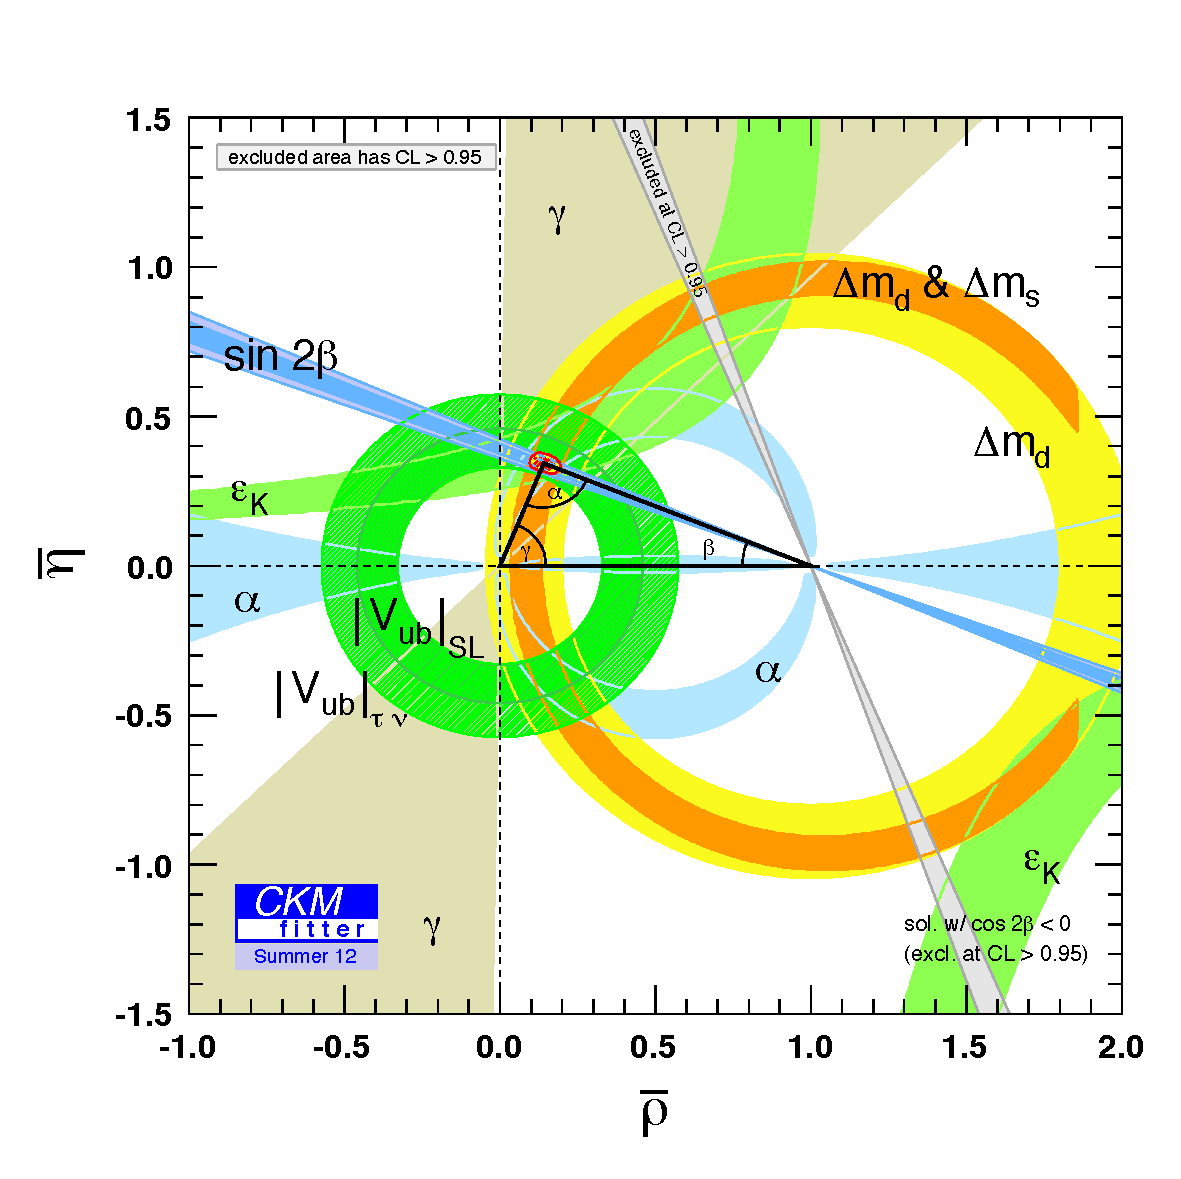
\includegraphics[width=1.0\textwidth]{CKMfit.pdf} 
        \vspace{0.0cm}
   \hspace{1cm}\tiny{[1] CKMfitter Group, J. Charles et al. ICHEP conference (July 2012)}
  \end{center}
    \end{column}
  \end{columns}
}







 \frame{
 \frametitle{2 - Inclusive Measurements of $V_{ub}$} 
\begin{itemize}
   \setlength{\itemsep}{12pt}
\item  $e^{+}e^{-}$ B factories BaBar and Belle:
$|V_{ub}| = (4.41 \pm 0.15 ^{+ 0.15} _{-0.17}) \times 10^{-3}$
\item Inclusive Approach:
   \begin{itemize}
       \setlength{\itemsep}{5pt}
  \item Measure partial branching fraction, $\Delta B (B \rightarrow X_{u} l^{-} \nu)$.
  \item Large background $B \rightarrow X_{c} l^{-} \nu$.
  \item Exploit kinematic endpoint of  $B \rightarrow X_{c} l^{-} \nu$.
  \item  Extrapolate to full phase space.
  \item Dominate uncertainty due to uncertainty on $m_{b}$.
  \end{itemize}
\end{itemize}

    
}


 \frame{
 \frametitle{2- Exclusive Measurements of $|V_{ub}|$} 


            \begin{columns}[T]
   \begin{column}{.5\textwidth}
   \begin{center}
\begin{itemize}
  \setlength{\itemsep}{12pt}
\item BaBar, Belle and CLEO: \\
$|V_{ub}| = (3.23 \pm 0.31) \times 10^{-3}$
  \item Exclusive Approach:
   \begin{itemize}
     \setlength{\itemsep}{5pt}
  \item Exclusive final state ($\bar{B}_{0} \rightarrow \pi^{+} \l^{-} \bar{\nu}_{l}$)
  \item $\frac{d \Gamma}{d q^{2}} = \frac{G_{F}^{2} |V_{ub}|^{2}}{24 \pi^{3}} |p_{\pi}|^{3} | f_{+} (q^{2})|^{2}$ 
  \item $ | f_{+} (q^{2})|^{2}$ predicted by lattice QCD
  \item Uncertainty dominated by $ | f_{+} (q^{2})|^{2}$.
  \end{itemize}
  \end{itemize}
  \end{center}
  \end{column}
      \begin{column}{.5\textwidth}
      % \footfullcite{gfgfg}

      
  \begin{center}
   \footnotesize{ \uline {Measured partial branching fraction  \\ $\Delta B (\bar{B}_{0} \rightarrow \pi^{+} \l^{-} \bar{\nu}_{l})$ [2]}:}
   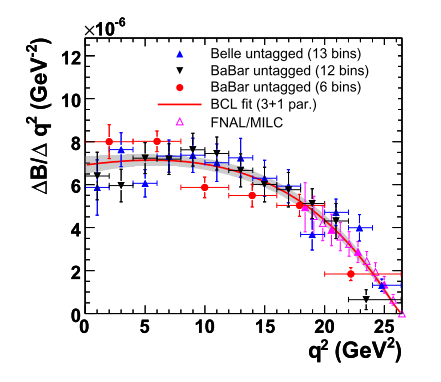
\includegraphics[width=1.0\textwidth]{BF2.png} 
\end{center}
    \end{column}
  \end{columns}

  \vspace{0.8cm}
   \tiny{[2] J. Beringer et al., Determination of $V_{ub}$ and $V_{cb}$ (Particle Data Group). \textit{Phys. Rev.} D\textbf{86}, 010001 (2012).}
}






 \frame{
 \frametitle{3 - $|V_{ub}|$ with LHCb }
 

 
 \begin{itemize}
  \item Large pion backgrounds.
  \item Other possible decays: $\Lambda_{b} \rightarrow p \mu^{-} \bar{\nu}_{\mu}$ and  $\bar{B}_{s} \rightarrow K^{+} \mu^{-} \bar{\nu}_{\mu}$
    \begin{center}
  
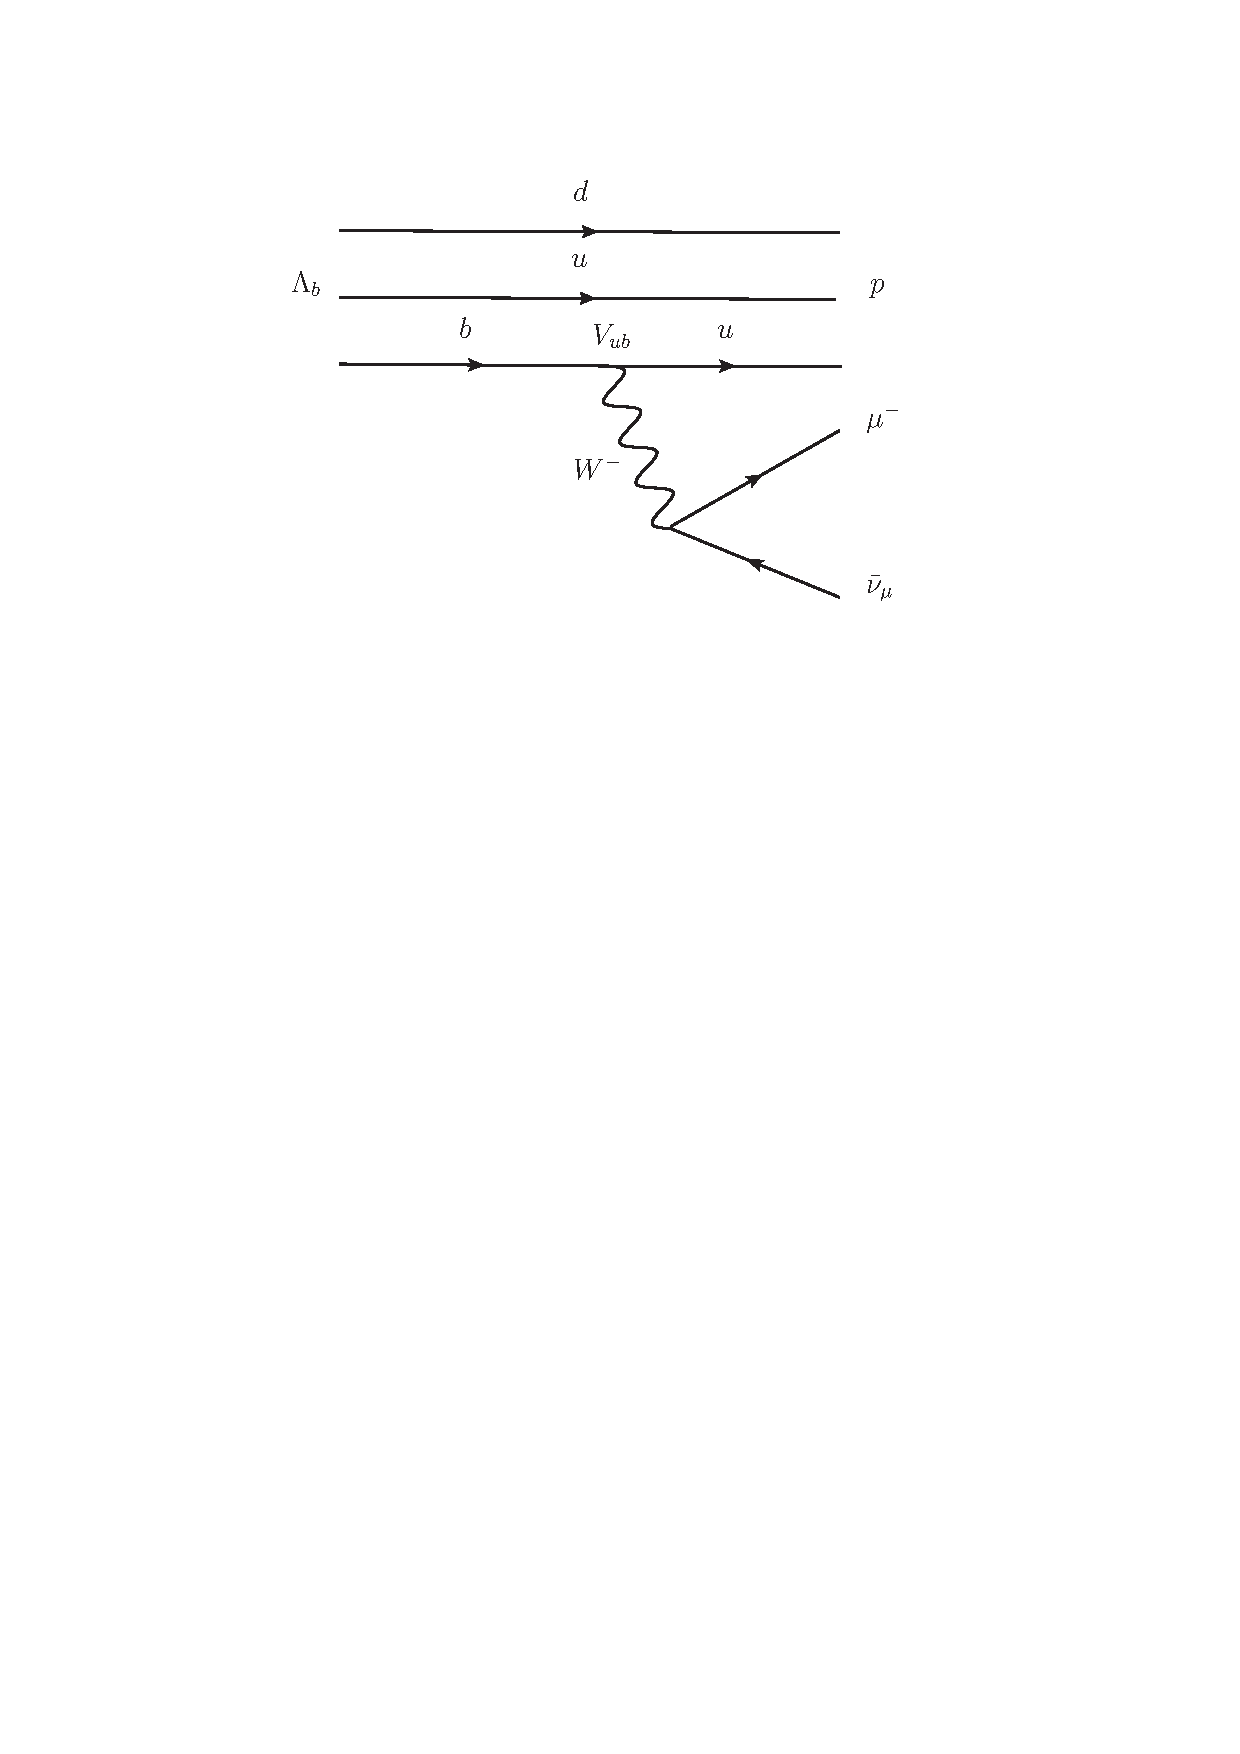
\includegraphics[trim = 15mm 190mm 0mm 30mm, clip, width=8cm]{feynsig.pdf} 

\end{center}
\item Advantages of $\Lambda_{b} \rightarrow p \mu^{-} \bar{\nu}_{\mu}$:
   \begin{itemize}
    \item $f_{\Lambda_{b}}/(f_{u}+f_{d}) \sim 0.40 $  and  $f_{\Lambda_{b}} /f_{s} \sim 3$
  \item Proton provides a more distinctive final-state.
  \end{itemize}
\end{itemize}

}

\frame{
 \frametitle{3 - $\Lambda_{b} \rightarrow p \mu^{-} \bar{\nu}_{\mu}$ with LHCb}

            \begin{columns}[T]
   \begin{column}{.5\textwidth}
   \begin{center}
    \begin{itemize}
      \setlength{\itemsep}{6pt}
   \item Displaced secondary vertex.
   \item  $\mu$ and $p$ tracks.
    \item Muon systems 
    %($p_{\text{T}\mu} > 1.3 $GeV/c)
   \item 2 RICH detectors for PID
    \item Proton, kaon and pion separation \\ $|\vec{p}| = 2 \rightarrow100$ GeV/c
       \end{itemize}
       \end{center}
  \end{column}
      \begin{column}{.5\textwidth}
      % \footfullcite{gfgfg
         \begin{center}
   \hspace{0.5cm} \footnotesize{\uline{Schematic of RICH 1:}}
  
   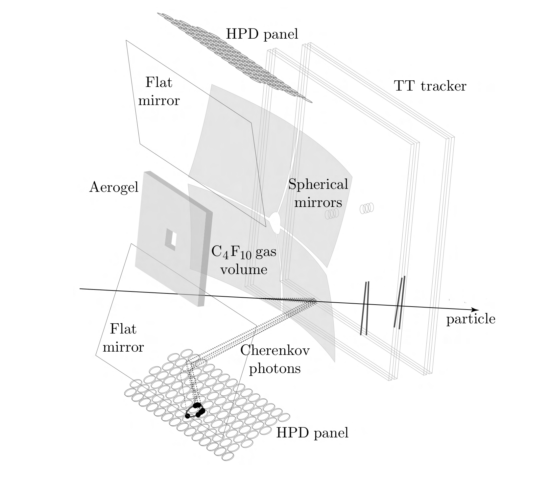
\includegraphics[width=1.2\textwidth]{RICH.png} 
 \end{center}
    \end{column}
  \end{columns}


}

 \frame{
 \frametitle{3 - RICH PID performance}

  \begin{center}
 
    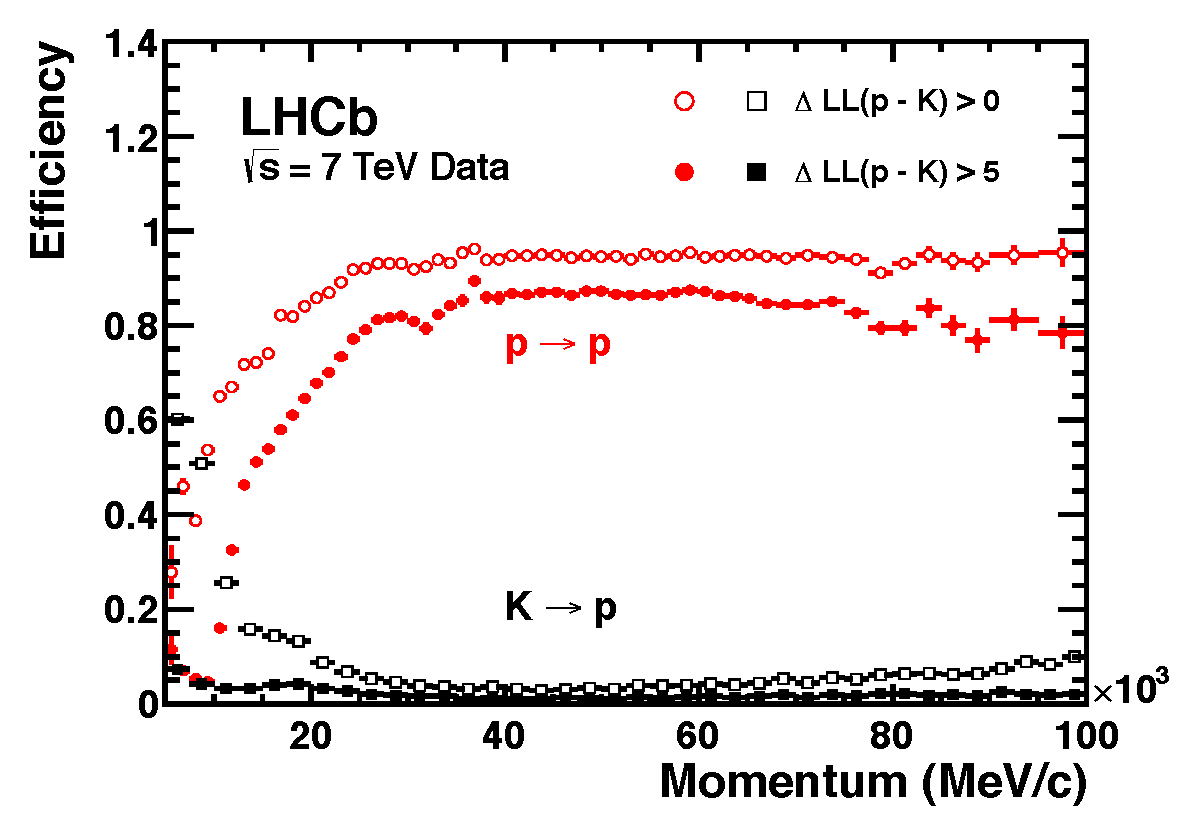
\includegraphics[width=0.5\textwidth]{pk.pdf}  
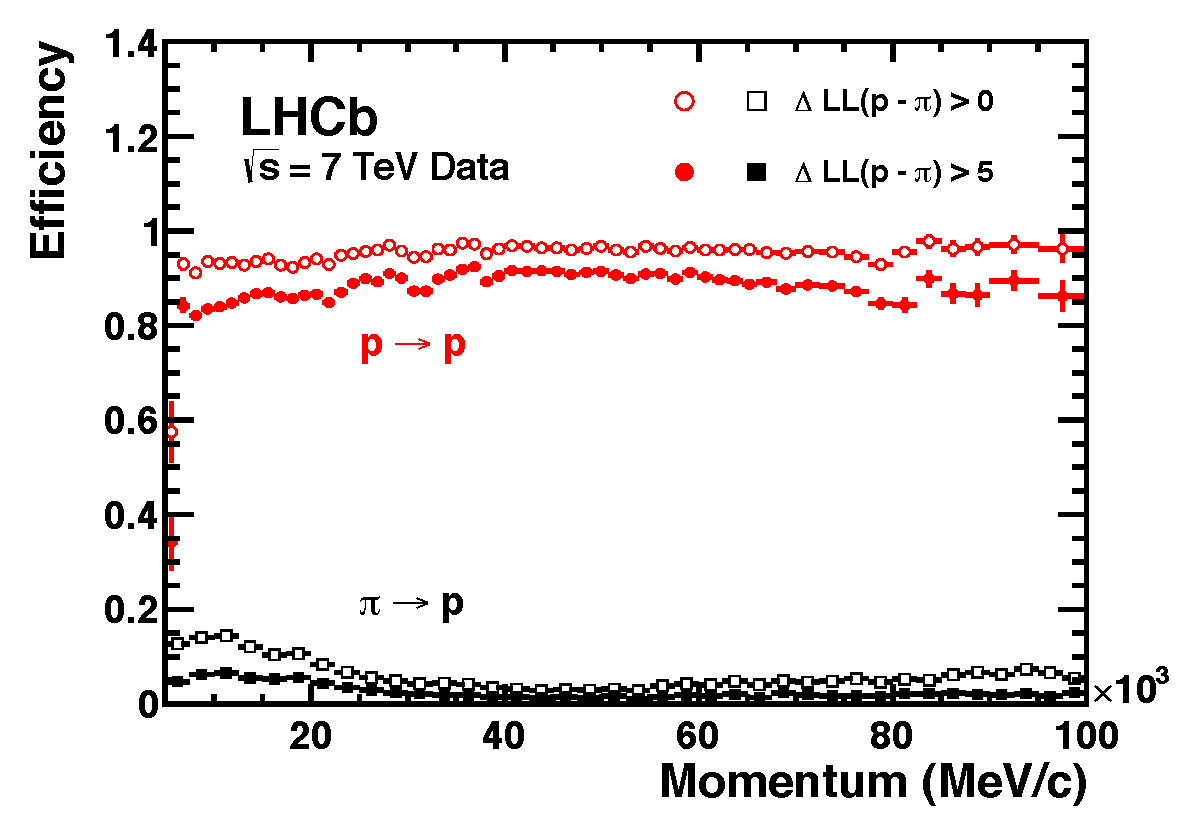
\includegraphics[width=0.5\textwidth]{pionp.pdf} 
\begin{itemize}

  \item High $K$-$p$ misidentification rate below $10$ GeV/c.
\end{itemize}
\end{center}

}

 \frame{\frametitle{4 - Initial Generator Level Studies} 
\begin{center} 
\begin{itemize}
\small

  \item Generator level sample of $pp$ to inclusive $B$ events.
  \begin{itemize} 
  \item At least one lepton with $p_{\rm{T}} > 1.5$ GeV/c.
    \end{itemize} 
  \item Search for $p$, $K^{+}$ and $\pi^{+}$ from the decay chain of a B hadron.

\end{itemize}
  \begin{center}
    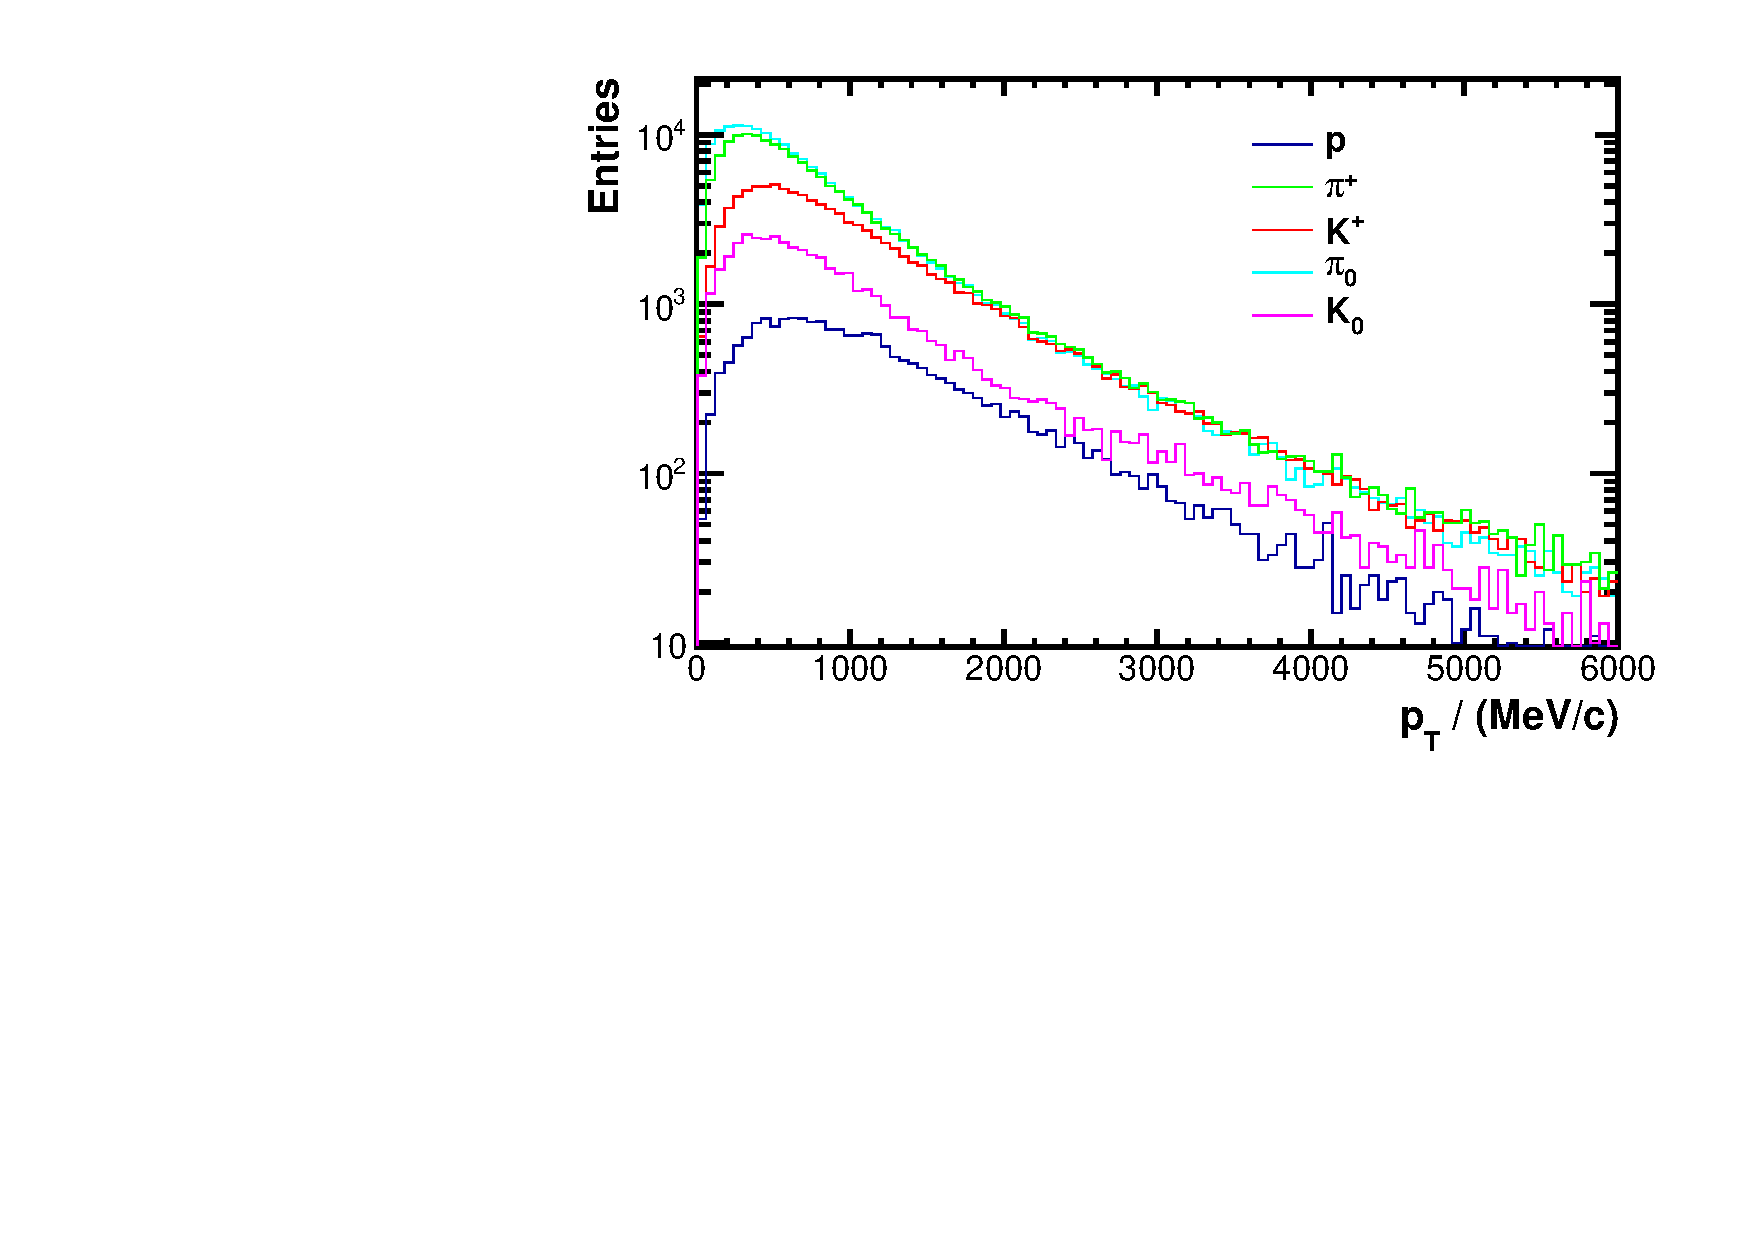
\includegraphics[width=0.50\textwidth]{production.pdf}  
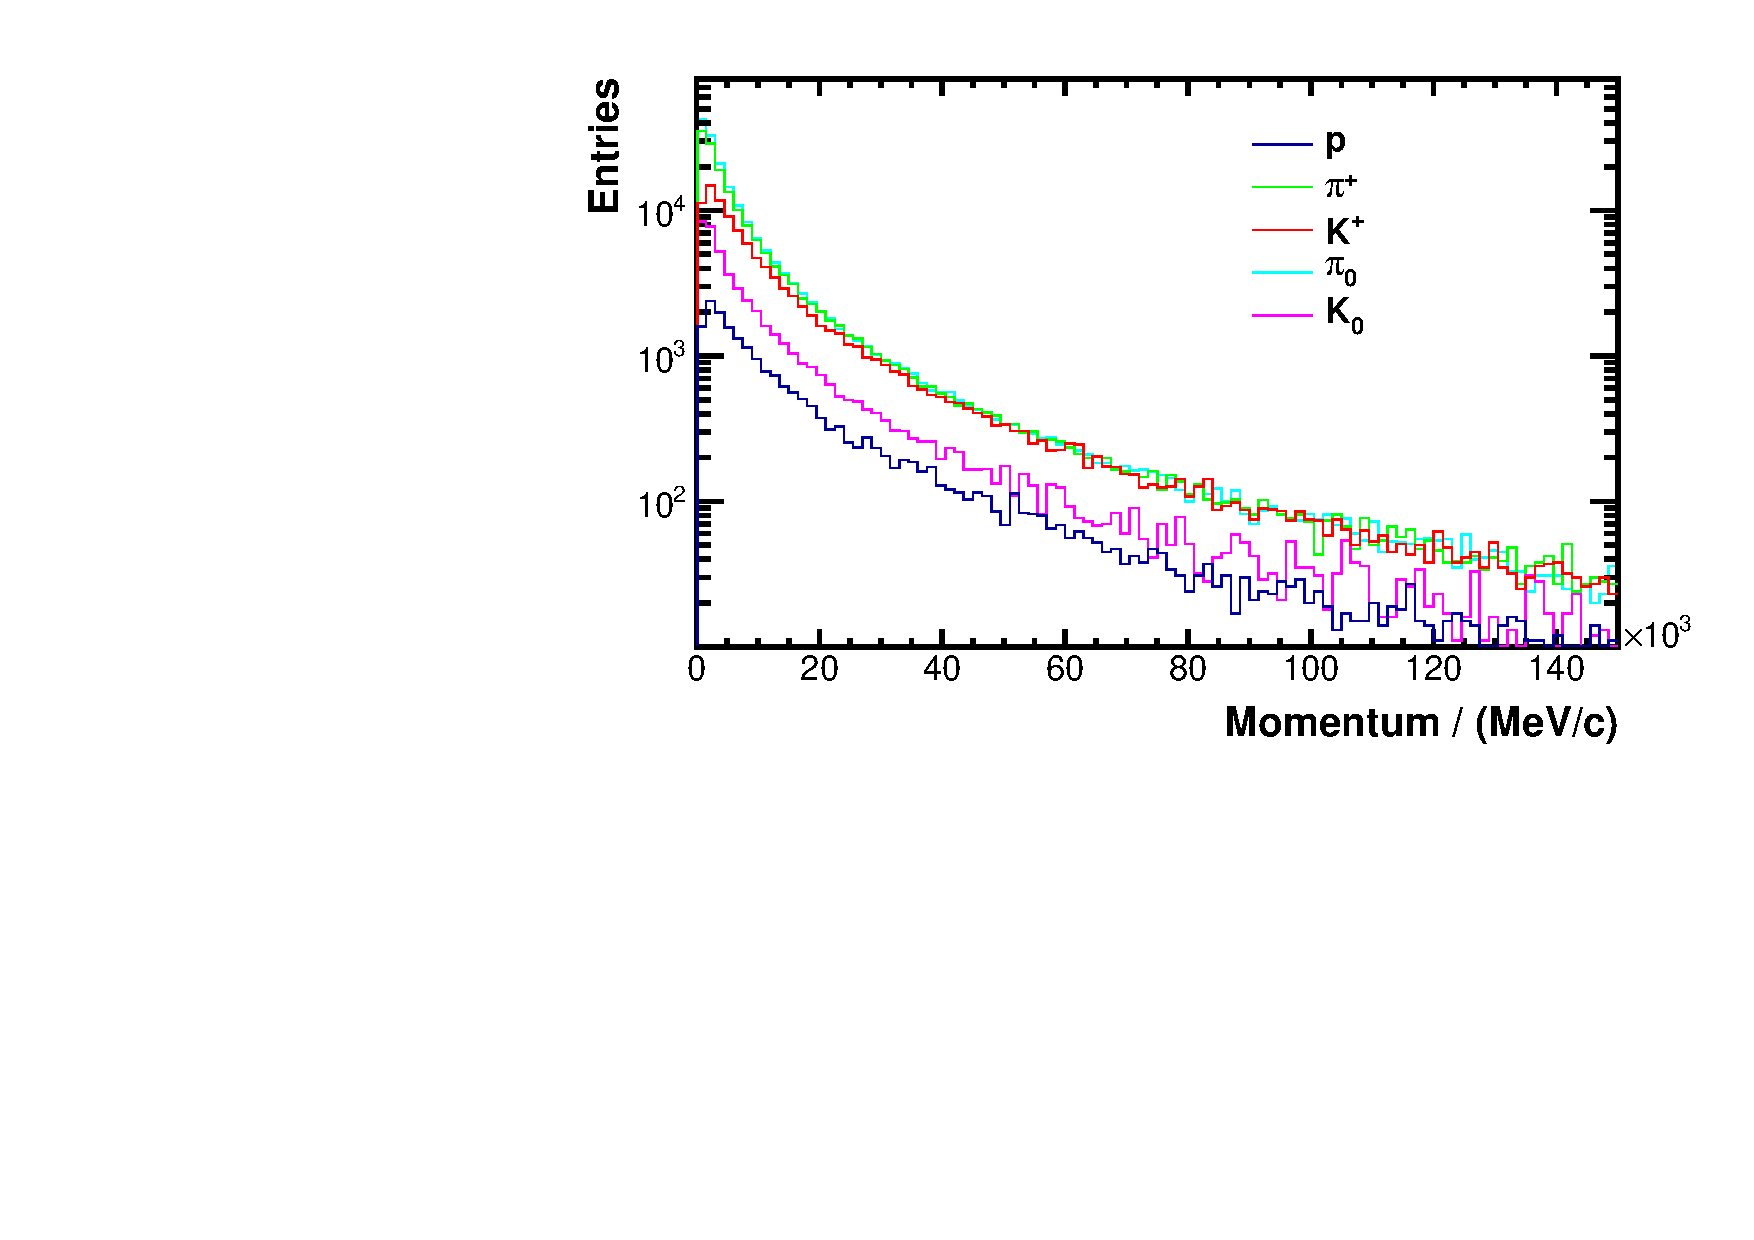
\includegraphics[width=0.50\textwidth]{production_p.pdf} 
\end{center}
\end{center} 


}

 \frame{\frametitle{} 
\begin{center} 
\begin{itemize}
\small
  \setlength{\itemsep}{6pt}
  \item Require $p$, $K^{+}$ and $\pi^{+}$ to vertex with a muon with $p_{\rm{T}}>1.5$ GeV/c.
  \item Plot signal samples of $\Lambda_{b} \rightarrow p \mu^{-} \bar{\nu}_{\mu}$ and $\bar{B}_{s} \rightarrow K^{+} \mu^{-} \bar{\nu}_{\mu}$
  \item  Weight signal samples using:
  \begin{itemize}
   \item $B (\Lambda_{b} \rightarrow p \mu^{-} \bar{\nu}_{\mu}) \approx B({B}_{s} \rightarrow K^{+} \mu^{-} \bar{\nu}_{\mu}) \sim 10^{-4}$
    \item Efficiencies of generator level cuts.
    \item $\Lambda_{b}$ and $B_{s}$ production fractions.
  \end{itemize}

\end{itemize}
    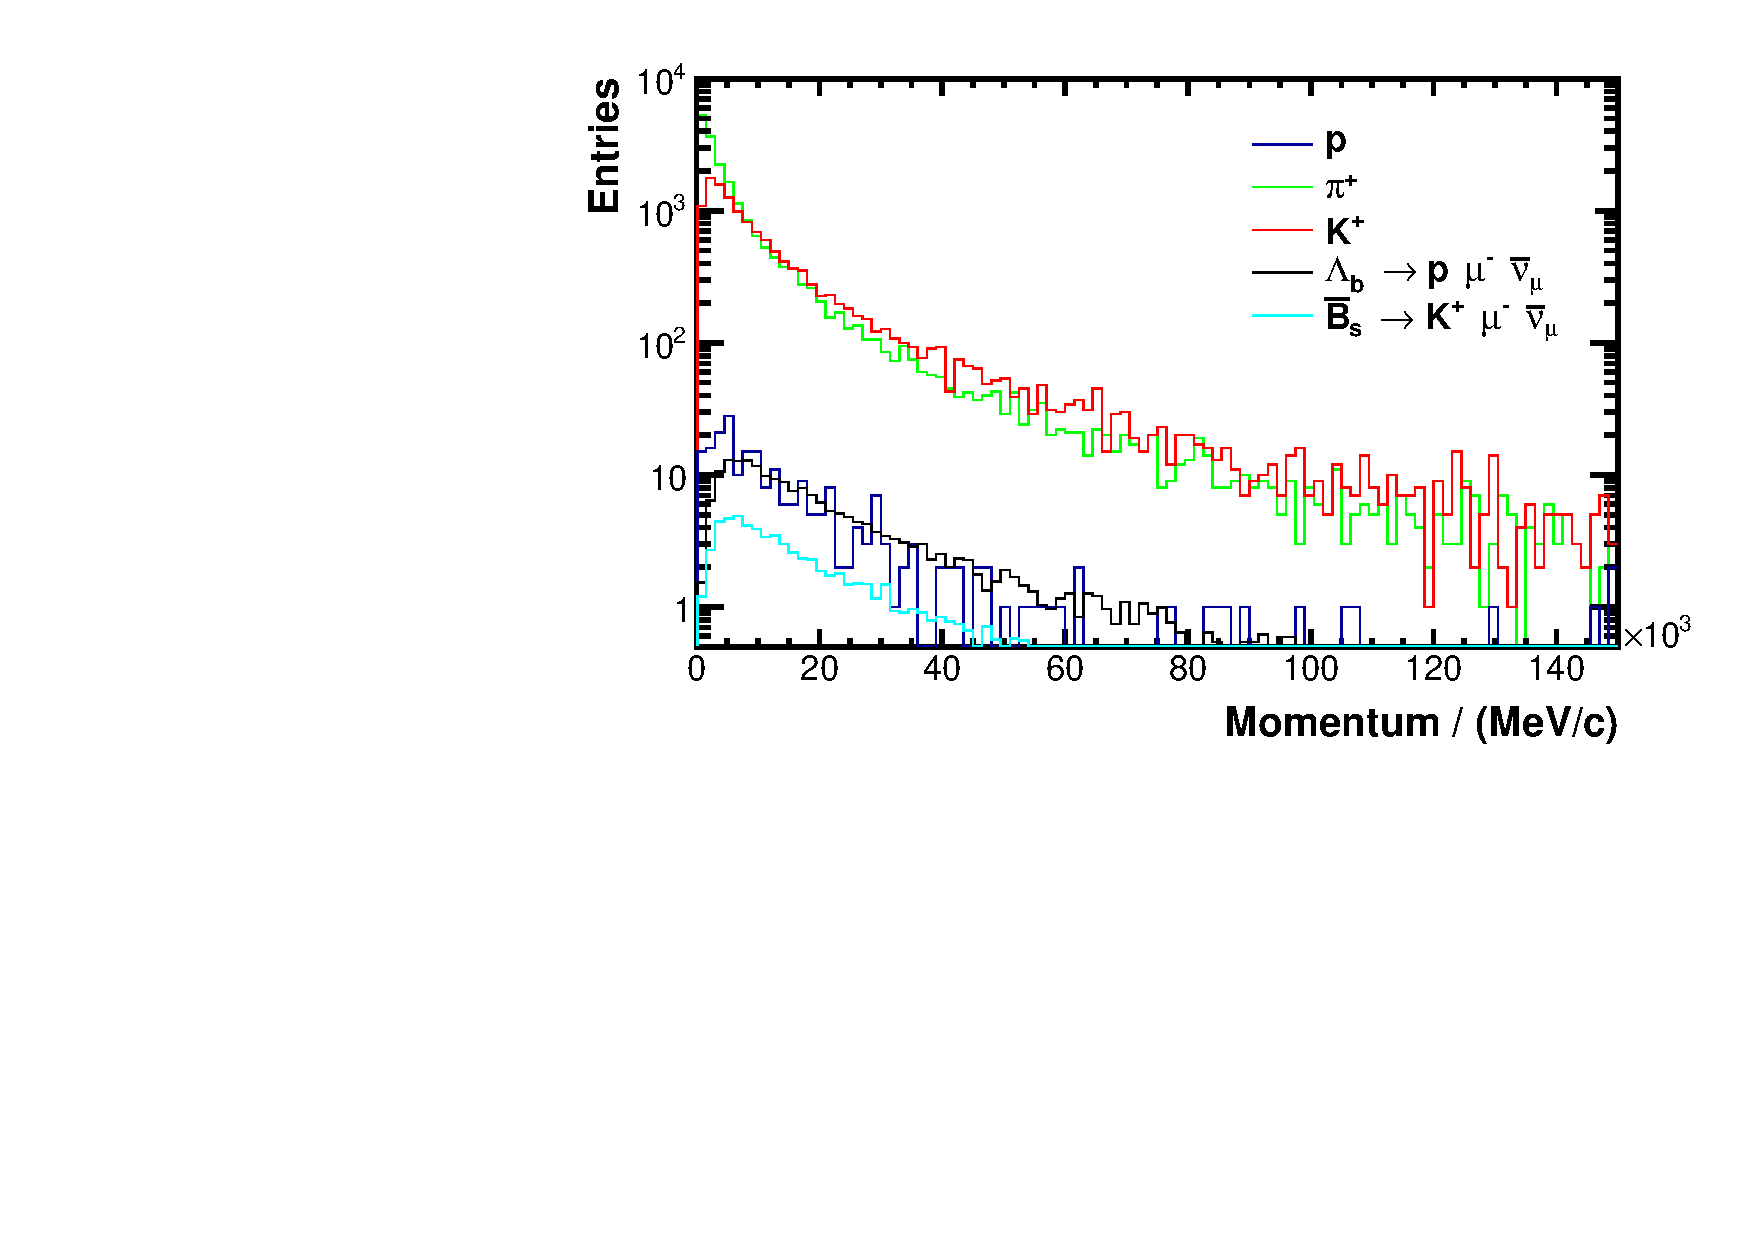
\includegraphics[width=0.7\textwidth]{Allp2.pdf}   
    % 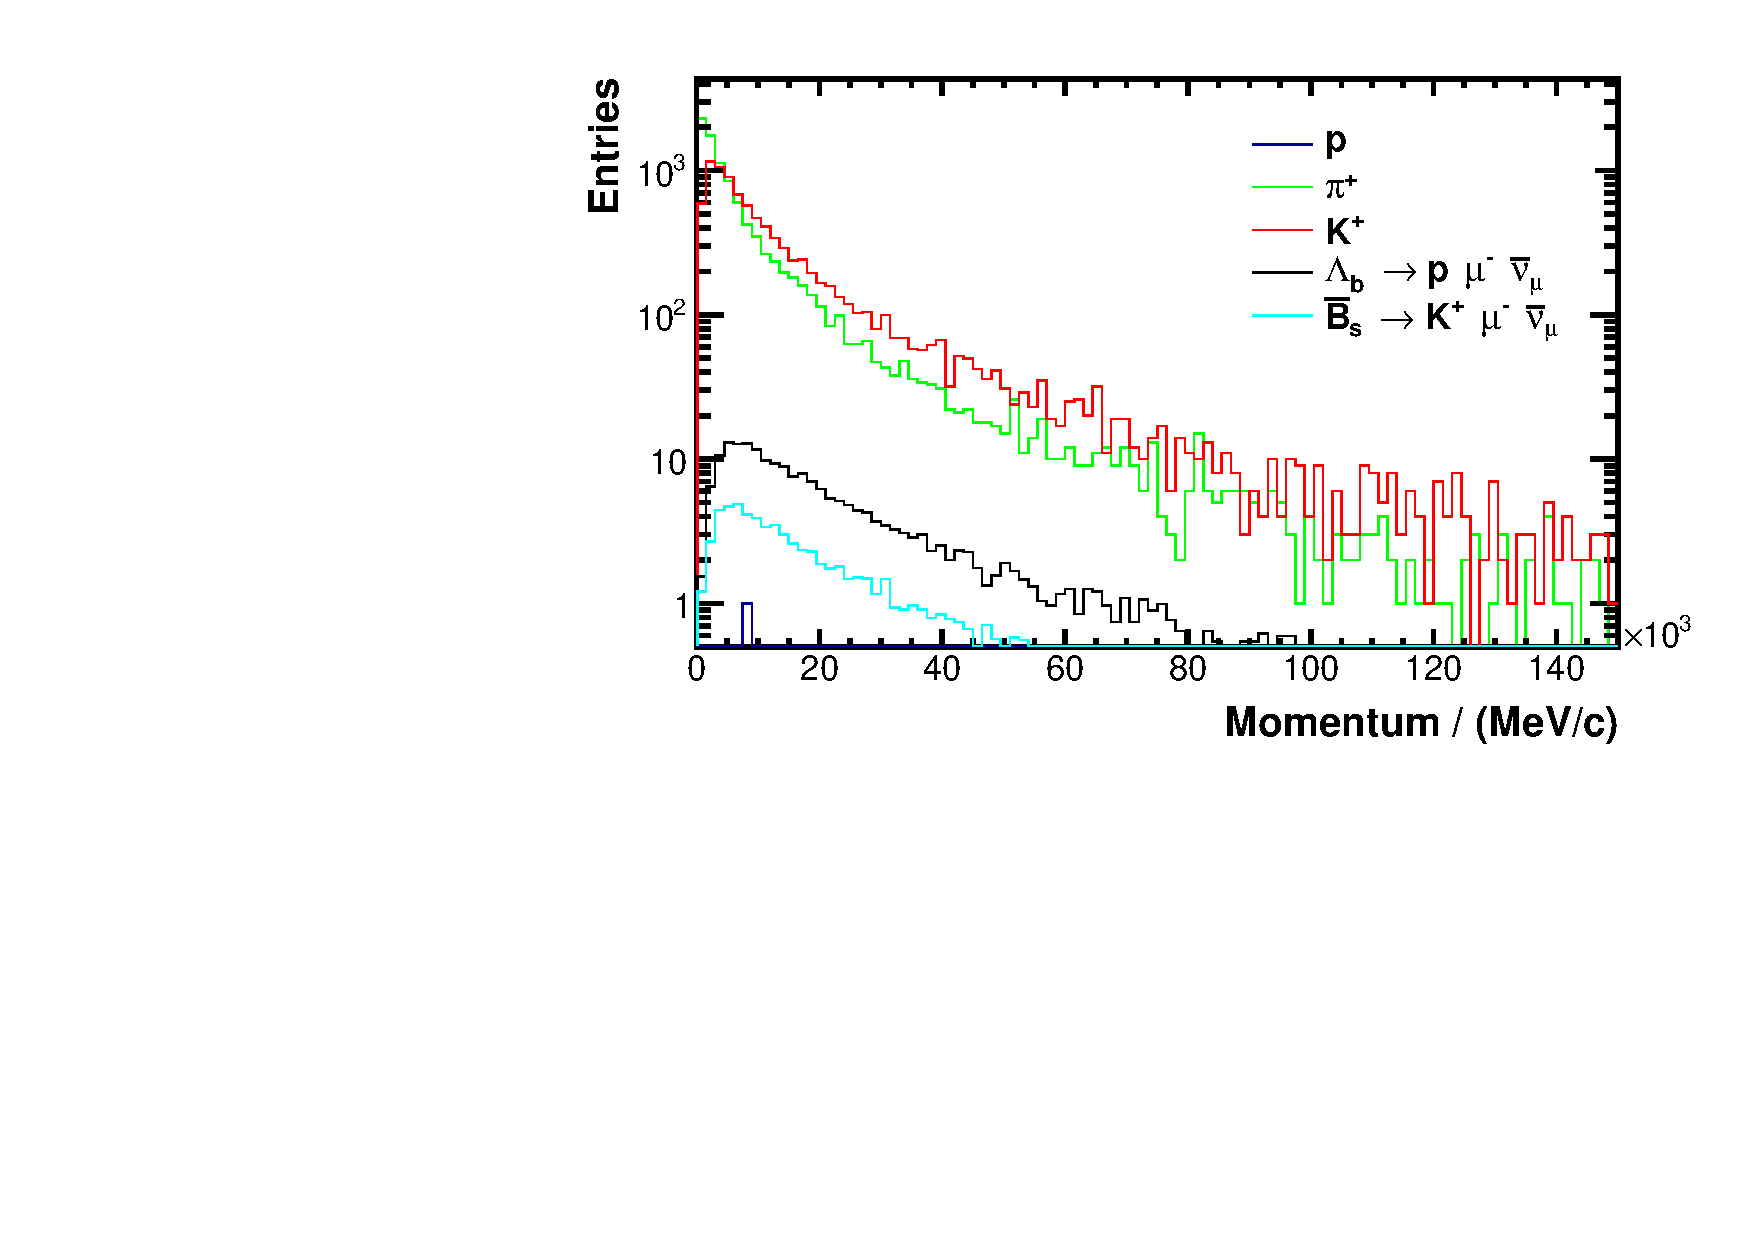
\includegraphics[width=0.5\textwidth]{Allp2_os.pdf} 
\end{center} 


}






 \frame{\frametitle{Conclusion} 
\begin{center} 

\begin{itemize}
  \setlength{\itemsep}{6pt}
\small
\item $|V_{ub}|$ is important constraining for CKM physics.
\item $\sim$$3\sigma$ discrepancy between exclusive and inclusive measurements.
\item Yet to be observed $\Lambda_{b} \rightarrow p \mu^{-} \bar{\nu}_{\mu}$ is a promising decay.
\item Generator level studies indicate that proton backgrounds are low.

\item Future Work:
\begin{itemize} 
\item Determine exact selection criteria for a measurement of $\Delta B (\Lambda_{b} \rightarrow p \mu^{-} \bar{\nu}_{\mu})$.
\end{itemize}
\end{itemize}
   
\end{center} 
}



 \frame{\frametitle{} 
\begin{center} 
Thanks for listening.  Any questions?
\end{center} 


}




 %\frame{\frametitle{Background theory} 
%\begin{itemize}
%\setlength{\itemsep}{10pt}
  %\item Yukawa interaction for quarks:
      %  \[
     % \Lagr_{Yukawa} = - Y_{ij}^{d} \bar{Q}_{Li} \phi  D_{Rj} - Y_{ij}^{u} \bar{Q}_{Li} \tilde{\phi} U_{Rj} + h.c
  % \]
  % where here $Q_{L}= \left(
%\begin{array}{c}
%u_{L}\\
%d_{L}\\
%\end{array}
%\right)$, $D_{R} = (d_{R})$, $U_{R} = (u_{R})$
%\item Transform quark fields via $U_{mn}^{u_{L}}, U_{mn}^{d_{L}}, U_{mn}^{u_{R}}, U_{mn}^{u_{R}}$ to get mass eigenstates ($u'_{nR}, u'_{nL}, d'_{nR}, d'_{nL}$)
%\item Charge Current interaction becomes:
    %    \[
    %  \Lagr_{CC} =     \frac{g}{2} u'_{Li} U_{ik}^{u_{L} }  \gamma^{\mu}  U_{kj}^{\dagger d_{L} } d'_{Rj} W^{+}_{\mu}+ h.c
   %\]
%\item $U_{ik}^{u_{L} }   U_{kj}^{\dagger d_{L} } = V^{CKM}_{ij}$
  %\item Well-structured.
%\end{itemize}
%}


 \end{document}
 
 
